\section {Kinematic Variables at Various Selection}
Figure~\ref{fig:kinAtEachSel700} show the kinematic distributions just before we apply a cut on them. The cuts shown are for the optimisation of 700 GeV resonanace. 
\newpage
\begin{figure}[h!]
\begin{center}
		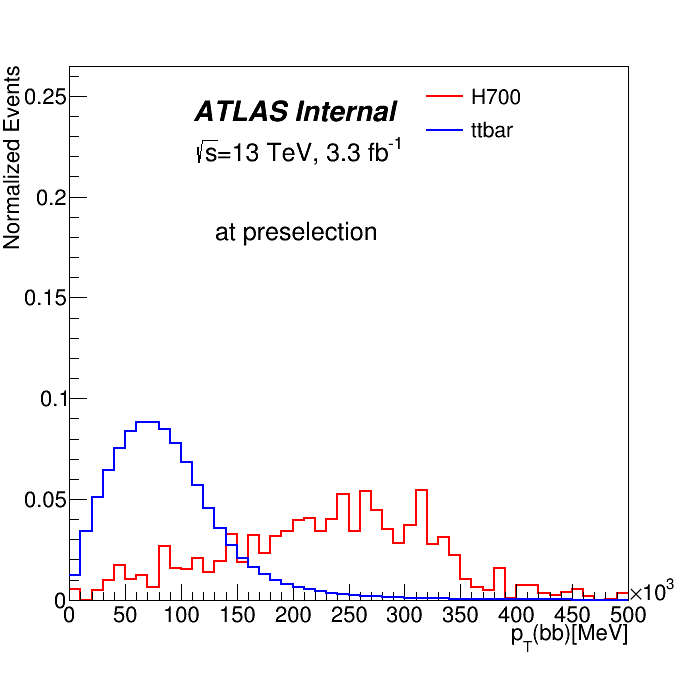
\includegraphics[height=60mm]{figures/kinAtEachSel700/PRE_ss_bbPt.png} 
		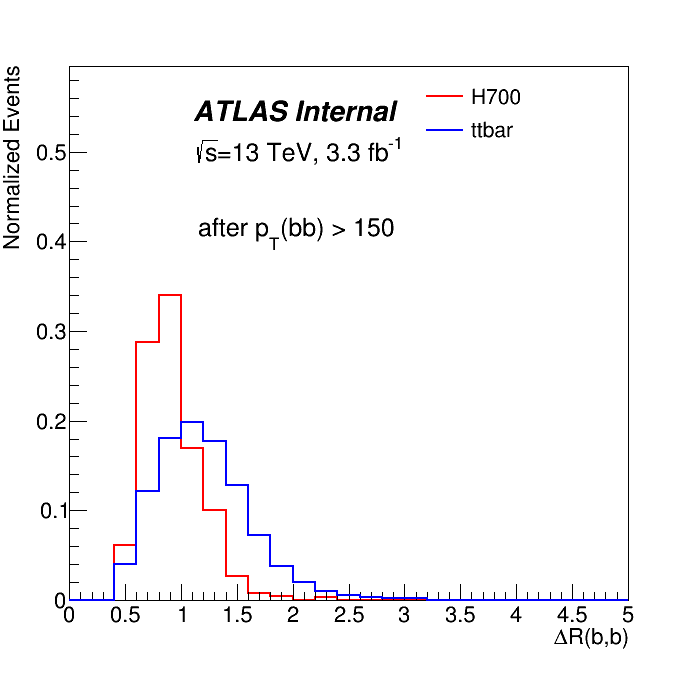
\includegraphics[height=60mm]{figures/kinAtEachSel700/SR_opt700_bbpt150_drbb.png}
		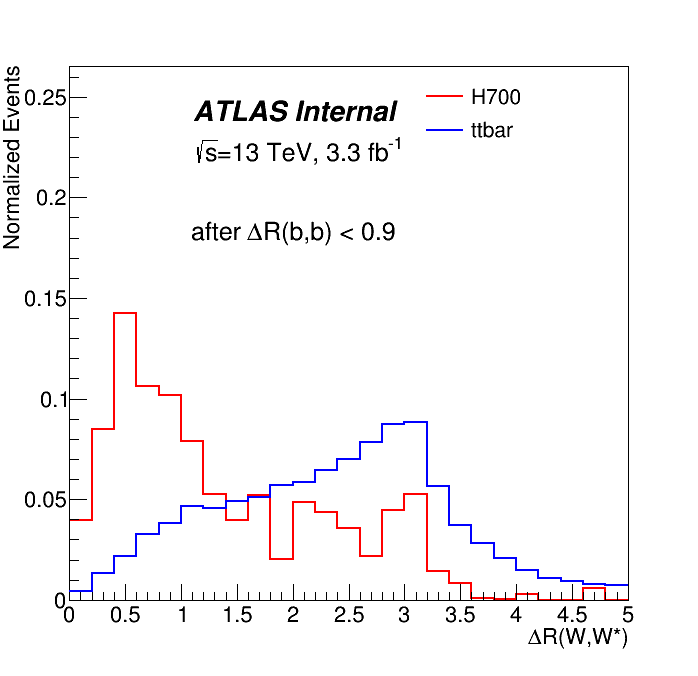
\includegraphics[height=60mm]{figures/kinAtEachSel700/SR_opt700_bbpt150_drbb09_drww.png} 
		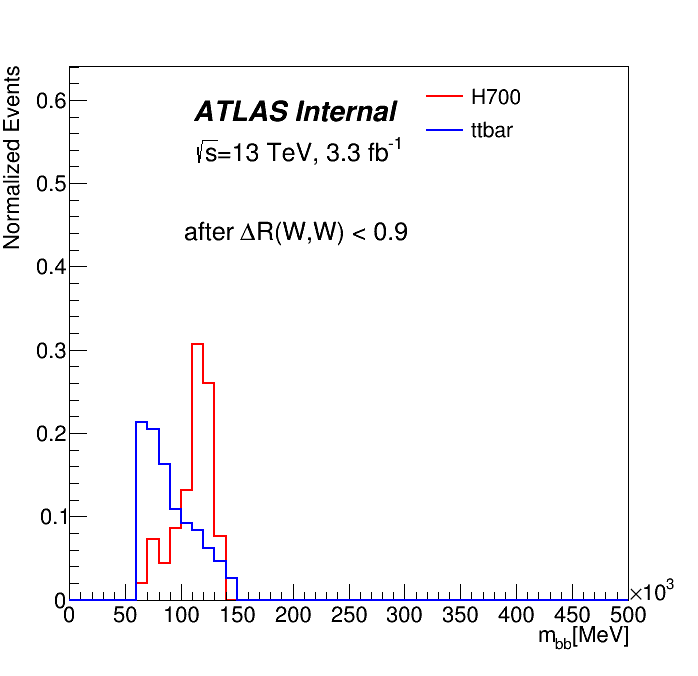
\includegraphics[height=60mm]{figures/kinAtEachSel700/SR_opt700_bbpt150_drbb09_drww09_bbMass.png}
		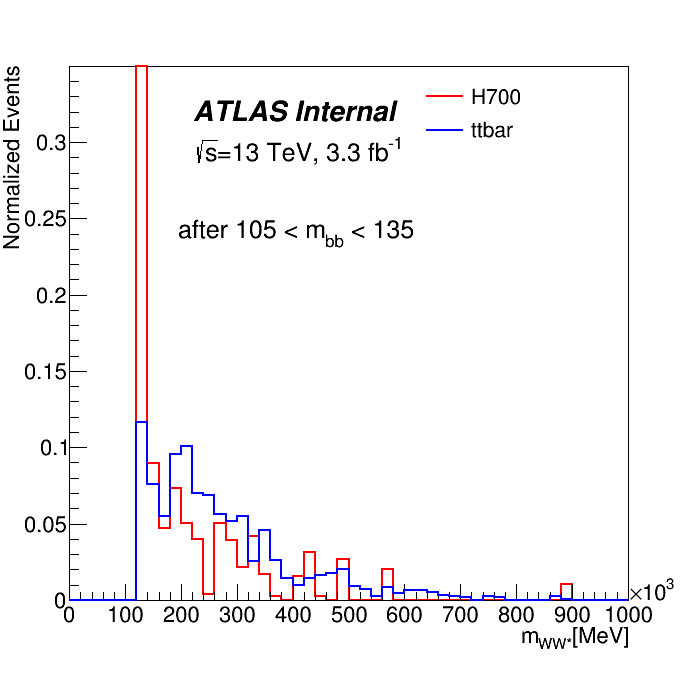
\includegraphics[height=60mm]{figures/kinAtEachSel700/SR_opt700_bbpt150_drbb09_drww09_mbb_WWMass.png} 
		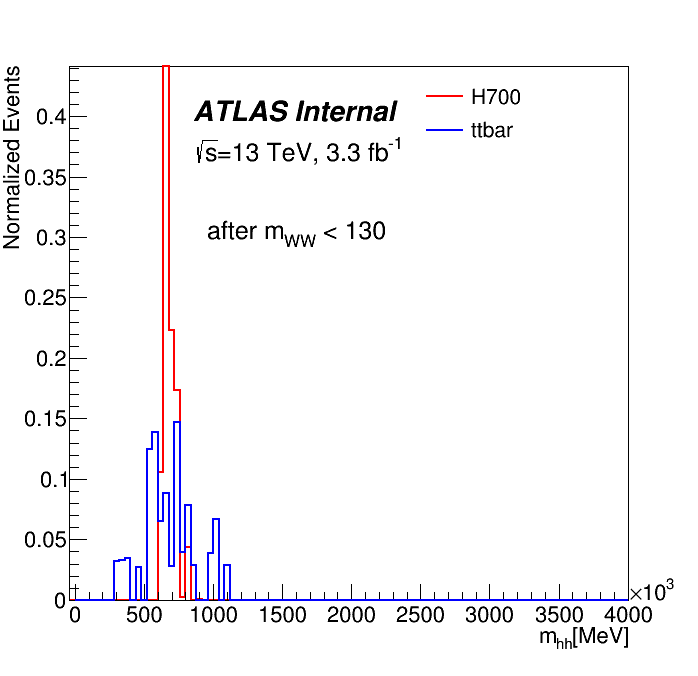
\includegraphics[height=60mm]{figures/kinAtEachSel700/SR_opt700_bbpt150_drbb09_drww09_mbb_mww_hhMass.png} 
%               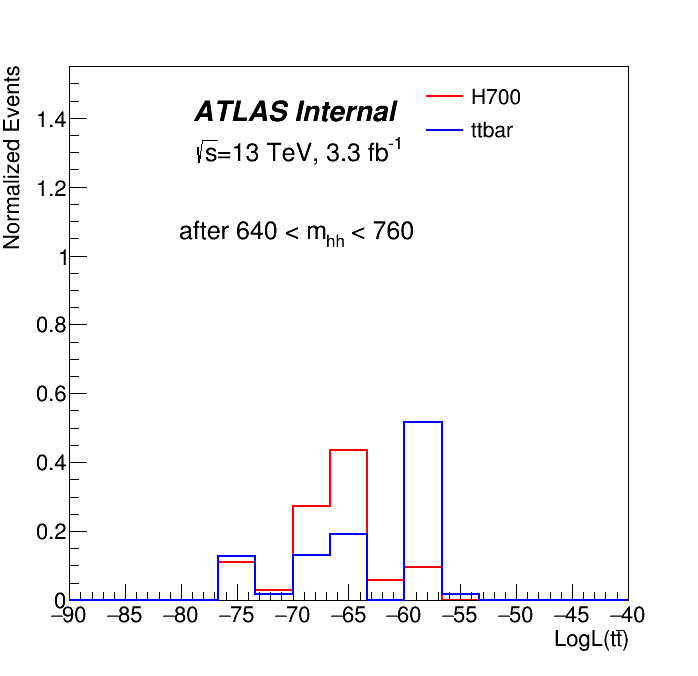
\includegraphics[height=65mm]{figures/kinAtEachSel700/SR_opt700_bbpt150_drbb09_drww09_mbb_mww_mhh_LogLikelihood_ttbar.png}
	\caption{Event  kinematic distributions at each selection stage but just before applying the cut on them. The distributions show the main difference between the signal and the background process.}
	\label{fig:kinAtEachSel700}
	\end{center}    
\end{figure}